\subsubsection{Q10.20 data 10312021 11092021 grouped by scenario}

\begin{comment}
               EFPR        EO      EFNR     n    pvalue
(frauth,)  0.488372  0.511628  0.453488  43.0  0.886426
(icu,)     0.611111  0.388889  0.625000  36.0  0.071389
(rent,)    0.397436  0.602564  0.487179  39.0  0.173035
\end{comment}

\begin{table}[h]
    \centering
    \begin{tabular}{|c|c|c|c|c|c|}
        \hline
        scenario & EFPR & EO & EFNR & n & p-value\\
        \hline
        frauth & 0.488 & \textbf{0.512} & 0.453 & 43.0 & 0.886\\
		icu & \textbf{0.611} & 0.389 & \textbf{0.625} & 36.0 & 0.071\\
		rent & 0.397 & \textbf{0.603} & 0.487 & 39.0 & 0.173\\
		
        \hline
    \end{tabular}
    \caption{Grouped by scenario}
    \label{tab:my_label}
\end{table}
\begin{figure}[h]
    \centering
    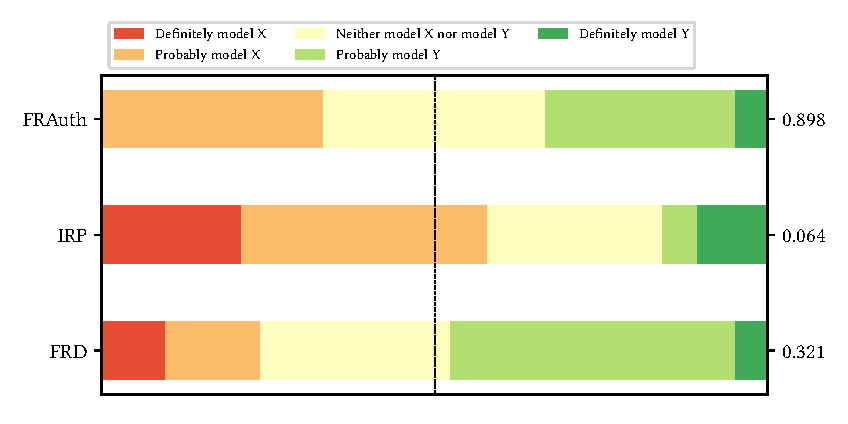
\includegraphics[width=0.8\textwidth]{figures/Q10.20/10312021_11092021/Q10.20_scenario.pdf}
    \caption{Grouped by scenario}
    \label{fig:my_label}
\end{figure}
